\chapter{Estimador analogico} \chapterlabel{Informe/5-EstimadorAnalogico} \label{cap:Estimador Analogico}

\section{Diseño y modelado del estimador analogico}

\noindent Para controlar la distancia de separaci\'{o}n del entrehierro del electroim\'{a}n es necesario conocer el gap de aire para poder realimentarlo en el lazo de control.  Para ello, se utiliza un estimador de posici\'{o}n que aprovecha la forma de onda triangular de la corriente que circula por el electroim\'{a}n. 



\noindent Para estimar la distancia se hace la derivada de la corriente, puesto que las pendientes de crecimiento y decrecimiento var\'{i}an con la separaci\'{o}n. Es importante tener en cuenta que durante el dise\~{n}o de la etapa de controlador de corriente, se eligi\'{o} una topolog\'{i}a que mantiene el sistema conmutando cont\'{i}nuamente (incluso para corriente nula) para tener siempre una estimaci\'{o}n disponible.



\noindent Se implementa un estimador compuesto por los bloques mostrados en la figura \ref{fig:img_Diagrama-Bloques-Estimador.png}. Se ingresa con una tensi\'{o}n triangular (ViL) que es la salida del sensor de efecto Hall. Para eliminar las componentes de alta frecuencia se aplica un filtro pasa bajos dejando pasar hasta la quinta arm\'{o}nica. Esta se\~{n}al filtrada conserva la forma triangular de la corriente. 

\noindent Al ingresar al derivador con ViL, la forma de onda resultante a su salida es aproximadamente cuadrada, y sus valores de alto y bajo se corresponden con las pendientes de bajada y subida multiplicadas por una constante de tiempo del derivador. Estas pendientes deber\'{i}an ser sim\'{e}tricas alrededor del punto de operaci\'{o}n de 2.5V, pero no lo son debido a la resistencia interna del electroim\'{a}n, que provoca que la pendiente de bajada sea mayor (en m\'{o}dulo) que la de subida. Por ello, se implementa la compensaci\'{o}n I*R, cuya salida ingresa al derivador y logra mantener la simetr\'{i}a alrededor de 2.5V. Esta se\~{n}al ingresa al \'{u}ltimo bloque que rectifica y filtra la forma de onda, obteni\'{e}ndose una tensi\'{o}n continua (Vout) proporcional a la distancia de separaci\'{o}n del gap ($Y_{g}$).

\begin{figure}[H]
	\centering
	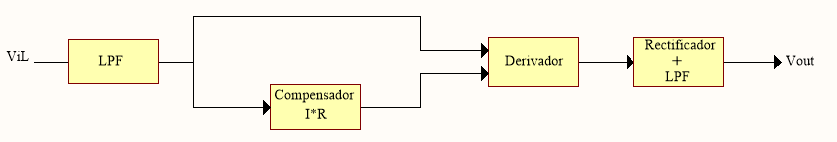
\includegraphics[scale=0.5]{Diagrama-Bloques-Estimador.png}
	\caption{Diagrama en Bloques del Estimador.}
	\label{fig:img_Diagrama-Bloques-Estimador.png}
\end{figure}

\subsection{An\'{a}lisis de la estimaci\'{o}n}

\noindent La ecuaci\'{o}n que gobierna la corriente en el electroim\'{a}n se puede calcular con las leyes de Kirchoff correspondientes al circuito que se ve en la figura \ref{fig:img_Circuito-electroimán-con-driver-corriente.png} y la expresión de la inductancia \ref{eq_inductancia_vs_y}.

\begin{figure}[H]
	\centering
	\includegraphics[scale=0.9]{Circuito-electroimán-con-driver-corriente.png}
	\caption{Circuito del electroimán con el driver de corriente.}
	\label{fig:img_Circuito-electroimán-con-driver-corriente.png}
\end{figure} 

\noindent Al resolver el circuito se obtiene:
\begin{equation} \label{eq_VbusCondicion}
	\pm V_{BUS}-\ L(Y_g)*\left|\frac{{di}_L}{dt}\right|-L_{\infty }*\left|\frac{{di}_L}{dt}\right|-R_L*I_L=0
\end{equation}


\noindent Se asume que:

\begin{equation} \label{eq_Derivadadi-dt}
	V_{BUS}>>i_L*R_L
\end{equation}
 
\noindent Se aproxima la derivada de la corriente como:

\begin{equation} \label{eq_derivadaAproximacion}
	\left|\frac{{di}_L}{dt}\right|\simeq \frac{V_{BUS}}{L(Y_g)+L_{\infty }}=\frac{V_{BUS}}{L_T(Y_g)}
\end{equation}

\noindent Seg\'{u}n mediciones realizadas, se tienen los valores de $L_T(Y_g)$ correspondientes a cada posici\'{o}n. En base a ellos se hace una aproximaci\'{o}n lineal para obtener la expresi\'{o}n de la derivada de la ecuaci\'{o}n \ref{eq_derivadaAproximacion}.

\noindent 

\begin{equation} \label{eq_di-dt_lineal}
{\left|\frac{{di}_L}{dt}\right|}_{Lineal}=\ 194690\ *\ Y[m]+676\ A/s
\end{equation}

\subsection{Modelo circuital del estimador de posici\'{o}n}

\noindent Para poder obtener $\left|\frac{{di}_L}{dt}\right|$ se utiliza un circuito derivador con un amplificador operacional como se observa en la figura  \ref{fig:img_Circuito-derivador}.

\begin{figure}[H]
	\centering
	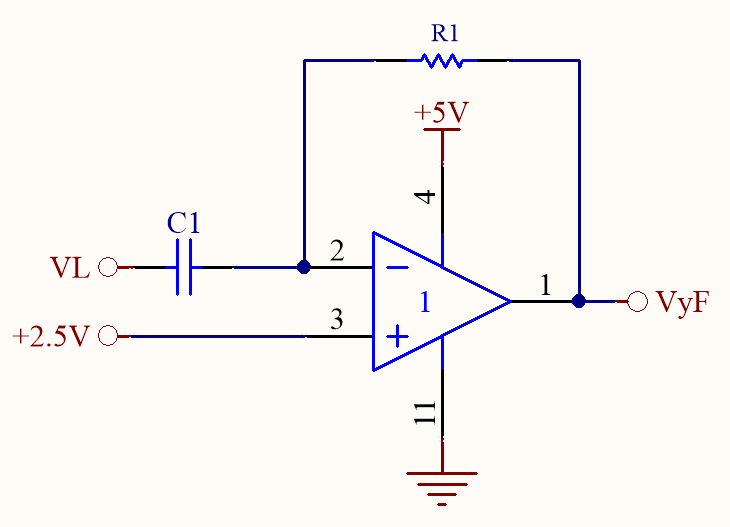
\includegraphics[scale=0.6]{Circuito-derivador.png}
	\caption{Circuito derivador.}
	\label{fig:img_Circuito-derivador}
\end{figure}

\noindent La salida del circuito, $V_{yf}(t)$, ante una entrada $V_L$ es:

\begin{equation} \label{eq_vyf1}
	V_{yf}(t)\ =\ 2.5V\ -\ \frac{dV_L}{dt}*C_1*R_1
\end{equation}


\noindent Al considerar que $V_L=K_h*i_L$, con $K_h$ como la constante del sensor de efecto Hall, se obtiene: 

\begin{equation} \label{eq_vyf2}
	V_{yf}(t)\ =2.5V\ -\frac{diL}{dt}*K_h*C_1*R_1
\end{equation}

\noindent $V_{yf}(t)$ tiene variaciones alrededor del setpoint de 2.5 V. Por lo tanto, para evitar la saturaci\'{o}n del derivador se debe cumplir que:

\begin{equation} \label{eq_vyf3}
	\left|-\frac{diL}{dt}*K_h*C_1*R_1\right|\ \le 2.5V
\end{equation}

\noindent Por lo tanto, con la ecuaci\'{o}n \ref{eq_derivadaAproximacion} y \ref{eq_di-dt_lineal}:

\begin{equation} \label{eq_condicionC1-R1}
	C_1*R_1<=\frac{2.5\ V\ *L_{min}}{V_{BUS}*K_h}
\end{equation}

\noindent Con $L_{min}= L_T(5\: mm)= 14.9\: mH$ (teniendo en cuenta la inductancia de dispersi\'{o}n) se obtiene: 

\begin{equation} \label{eq_condicionC1-R1-2}
	C_1*R_1<=\ 29.1\ ms
\end{equation}

\noindent Este derivador tendr\'{a} como salida una onda pulsada, cuyo flanco superior  es proporcional a la pendiente de bajada de la corriente en el electroim\'{a}n, y el flanco inferior es proporcional a la pendiente de subida de la corriente. 

\noindent Para los c\'{a}lculos se utiliz\'{o} $C_1*R_1=\ 25\ mS$, para dar un margen y evitar la saturaci\'{o}n del amplificador operacional.  

\noindent Con la ecuaci\'{o}n \ref{eq_di-dt_lineal} y \ref{eq_vyf3}, y con una variaci\'{o}n en torno a 2.5V se obtiene:


\begin{equation} \label{eq_Vyf-lineal}
	Vyf(Y_g)\ =\ |Kh*C_1*R_1*di/dt)|\ +2.5V=0.2595*Y_g(mm)+3.4V
\end{equation}

\noindent Se puede observar en la tabla \ref{tab_Vyf_vs_y} que, para los posibles valores en los que el electroim\'{a}n trabajar\'{a}, el estimador posee un rango de salida ${\mathit{\Delta}{Vyf}_{Lineal}}(5-2\ mm)=\ 0.78\ V$.

\begin{table}[H]
	\begin{center}
		\begin{tabular}{| c | c |}
			\hline
			$Y_g[mm]$ & ${Vyf(Y_g)}_{Lineal}$\\ \hline
			2 & 3.92 \\ \hline 
			3 & 4.18 \\ \hline 
			4 & 4.44 \\ \hline 
			5 & 4.7 \\ \hline 
		\end{tabular}
		\caption{$V_{yf}$ en función de la posición.}
		\label{tab_Vyf_vs_y}
	\end{center}
\end{table}

\subsection{Circuito del derivador compensado}

\noindent Puesto que los circuitos derivadores pueden presentar inestabilidad a alta frecuencia, es necesario compensarlo agregando una resistencia en serie al capacitor, para que genere un cero en la transferencia de realimentaci\'{o}n (ecuación \ref{eq_Aw_2}), como se observa en la figura  \ref{fig:img_Circuito_derivador_compensado}.

\begin{figure}[H]
	\centering
	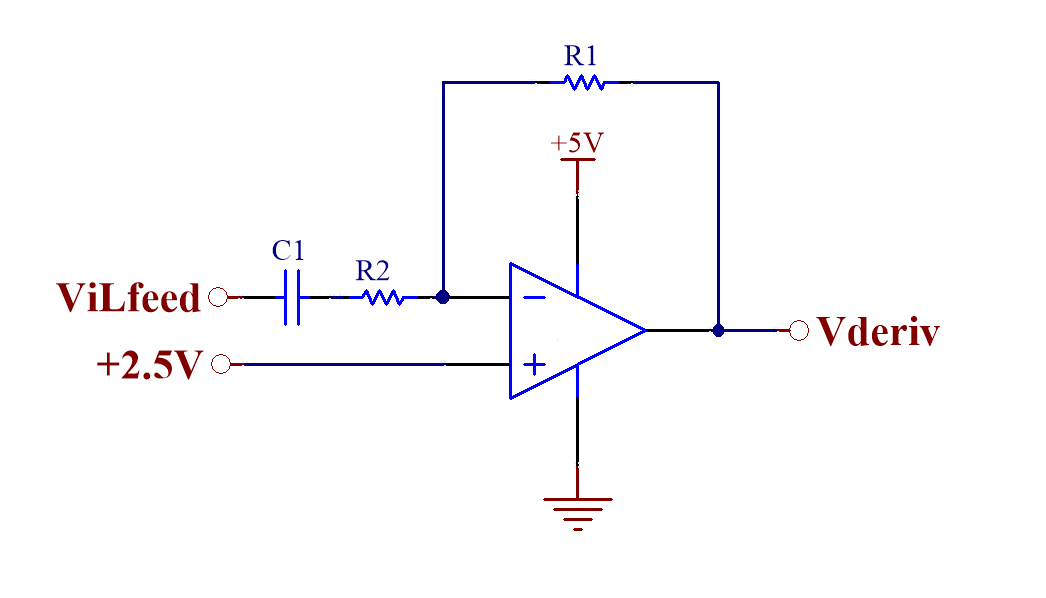
\includegraphics[scale=0.6]{Circuito-derivador- compensado.png}
	\caption{Circuito derivador compensado}
	\label{fig:img_Circuito_derivador_compensado}
\end{figure}

\noindent El operacional es internamente compensado, por lo que todos sus otros polos los tiene luego de el cruce por 0 dB de la ganancia. Para simplificar el an\'{a}lisis no se tienen en cuenta estos, ya que est\'{a}n fuera de la zona de inter\'{e}s.

\begin{equation} \label{eq_Aw_1}
	A(w)=\frac{1778279}{(\frac{s}{2\pi *20}+1)}
\end{equation} 

\begin{equation} \label{eq_Aw_2}
	\frac{1}{H(w)}=\frac{1+s*C_1*(R_1+R_2)}{1+s*C_1*R_2}\simeq \frac{1+s*C_1*R_1}{1+s*C_1*R_2}
\end{equation}

\noindent Para compensar el circuito se coloca un polo en 16 kHz, dando como resultado $R2=10\ ohm$, $C1=1\ uF$ y $R1=25\ kOhm\ $y un margen de fase de $\phi =49.6{}^\circ $, como se puede observar en la figura \ref{fig:img_GH del derivador compensado}.

\begin{figure}[H]
	\centering
	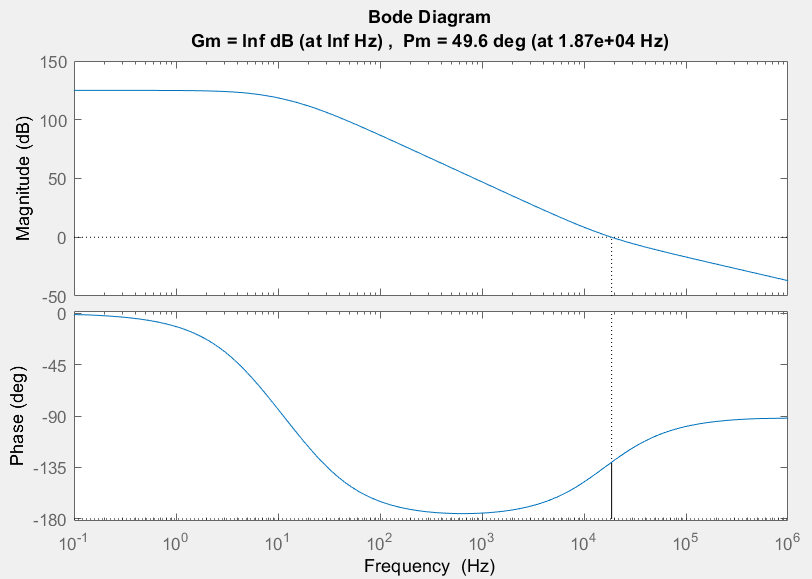
\includegraphics[scale=0.5]{GH-del-derivador-compensado.png}
	\caption{Transferencia a lazo abierto del derivador compensado.}
	\label{fig:img_GH del derivador compensado}
\end{figure}

\begin{figure}[H]
	\centering
	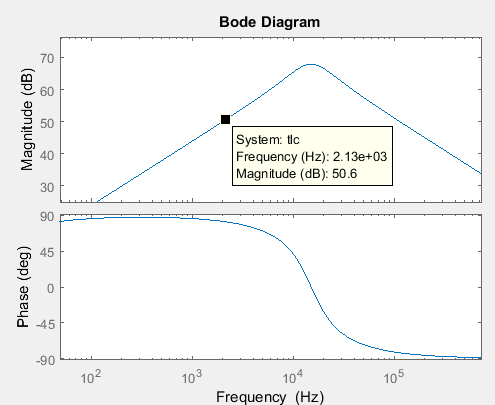
\includegraphics[scale=0.7]{Transferencia-de-lazo-cerrado.png}
	\caption{Transferencia de lazo cerrado.}
	\label{fig:img_Transferencia-de-lazo-cerrado}
\end{figure}

\noindent Como se observa en la figura \ref{fig:img_Transferencia-de-lazo-cerrado}la transferencia de lazo cerrado (TLC) tiene un comportamiento derivativo en las frecuencias cercanas a 2 kHz, como es deseado.

\noindent A continuaci\'{o}n se muestra la TLC del circuito derivador:
 
\begin{equation} \label{eq_Vyf-lineal}
	{Tlc}_{derivador}=\frac{V_{yf}}{Vil}=\frac{-0.025*s}{1+(\frac{2*0.473}{94,5\ krad/s})*s+(\frac{s}{94,5\ krad/s})^2}
\end{equation} 

\subsection{Dise\~{n}o del LPF}

\noindent Debido a que el derivador amplifica las se\~{n}ales de alta frecuencia es necesario agregar un filtro pasa bajos en su entrada. Como la se\~{n}al que va a ingresar al derivador es ViL, la cual es una onda triangular de frecuencia fundamental de 2KHz se dejar\'{a} pasar hasta la 5º arm\'{o}nica. Para su implementaci\'{o}n se utiliza un filtro activo Butterworth de orden 2, con una frecuencia de corte en 20 KHz. En la figura  \ref{fig:img_Filtro-para-la-entrada-del-derivador}se puede ver el filtro utilizado y en la figura \ref{fig:img_Respuesta-en-frecuencia-del-filtro-activo}, su respuesta en frecuencia.

\begin{figure}[H]
	\centering
	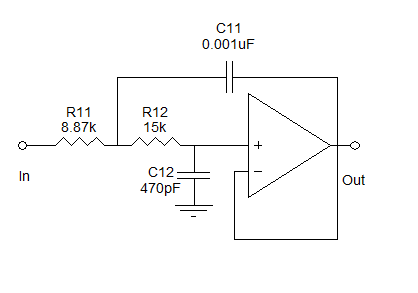
\includegraphics[scale=0.8]{Filtro-para-la-entrada-del-derivador.png}
	\caption{Filtro para la entrada del derivador.}
	\label{fig:img_Filtro-para-la-entrada-del-derivador}
\end{figure}

\begin{figure}[H]
	\centering
	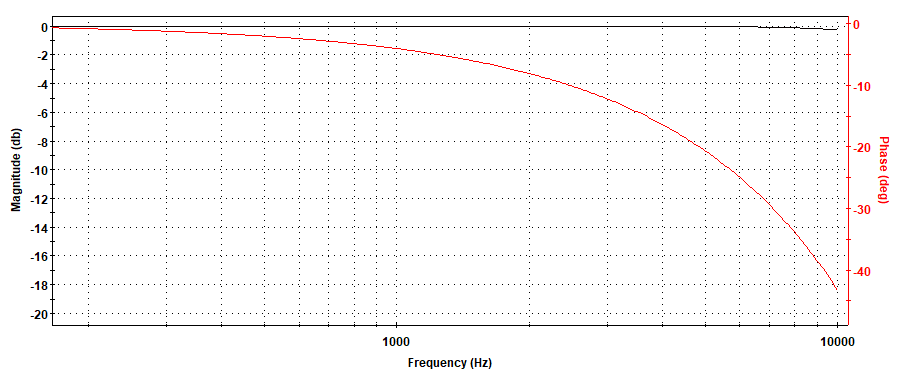
\includegraphics[scale=0.5]{Respuesta-en-frecuencia-del-filtro-activo.png}
	\caption{Respuesta en frecuencia del filtro activo.}
	\label{fig:img_Respuesta-en-frecuencia-del-filtro-activo}
\end{figure}

\subsection{Compensaci\'{o}n I*R}

\noindent Al circular corriente siempre en el mismo sentido por el electroim\'{a}n, se produce una ca\'{i}da de tensi\'{o}n casi constante en la resistencia interna, haciendo que no siempre est\'{e}n aplicados $\pm 24V$ al electroim\'{a}n sino que durante el $T_{ON}$ se aplican $24V-I*R$ y durante el $T_{OFF}$ se aplican $-24V-I*R$, haciendo que las pendientes sean distintas.

\begin{equation} \label{eq_Vbus-didt-RL}
\pm V_{BUS}-L(y)*\left|\frac{{di}_L}{dt}\right|-L_{\infty }*\left|\frac{{di}_L}{dt}\right|-R_L*I_L=0
\end{equation}

\noindent C\'{o}mo  $R_L=0.2\ \mathit{\Omega}$ y suponiendo una corriente de $21\ A$

\begin{equation} \label{eq_Vbus-didt-RL-2}
\pm V_{BUS}-R_L*I_L=\ \pm 24-4.2
\end{equation}

\noindent Por lo tanto, para $V_{BUS}=24\ V$:

\begin{equation} \label{eq_Vbus-didt-RL-3}
	V_{BUS}-R_L*I_L=\ +24-4.2=\ 19.8V
\end{equation}

\noindent Para $V_{BUS}=-24\ V$

\begin{equation} \label{eq_Vbus-didt-RL-4}
	V_{BUS}-R_L*I_L=\ -24-4.2=\ 28.2V
\end{equation}

\noindent Por lo tanto, sobre el electroim\'{a}n se aplicar\'{a}n dos tensiones distintas, en valor absoluto, durante la carga y descarga. Esto provoca que la rampa de corriente sea asim\'{e}trica.

\noindent Como luego se utilizar\'{a} un rectificador de onda completa, se desea que la rectificaci\'{o}n de cada una de estas pendientes resulte en el mismo valor. En la figura \ref{fig:img_Forma-de-onda-luego-de-rectificar-sin-compensación-IR} se muestra el efecto luego de la rectificaci\'{o}n sin realizar ninguna compensaci\'{o}n:
\colorbox{yellow}{Ver si esta imagen queda mejor con fondo blanco}
\begin{figure}[H]
	\centering
	\includegraphics[scale=0.5]{Forma-de-onda-luego-de-rectificar-sin-compensación-IR.png}
	\caption{Forma de onda luego de rectificar sin compensación IR.}
	\label{fig:img_Forma-de-onda-luego-de-rectificar-sin-compensación-IR}
\end{figure}

\noindent Se busca corregir esto en la estimaci\'{o}n variando el setpoint de la salida del derivador. Para lograrlo se debe cambiar la tensi\'{o}n en la entrada figura no inversora ($V_{bias}$) como se muestra en la figura \ref{fig:img_Esquema-circuital-del-derivador}. 

\begin{figure}[H]
	\centering
	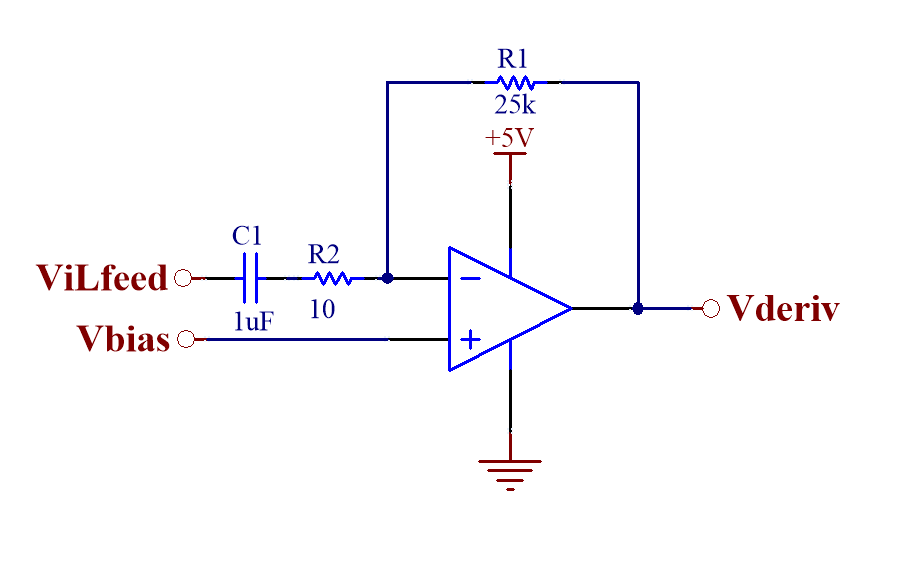
\includegraphics[scale=0.6]{Esquema-circuital-del-derivador.png}
	\caption{Esquema circuital del derivador.}
	\label{fig:img_Esquema-circuital-del-derivador}
\end{figure}

\noindent Se tiene que la pendiente de bajada de la onda triangular, en m\'{o}dulo, es mayor que la de subida. Por lo tanto, al derivar (con la inversi\'{o}n de signo), esta quedar\'{a} por encima del setpoint, y la pendiente de subida quedar\'{a} por debajo. Se debe compensar ese setpoint para que la forma de onda sea sim\'{e}trica alrededor de 2.5 V. 

\noindent Para la pendiente de bajada, la salida del derivador ser\'{a}:

\begin{equation} \label{eq_Vyf-Vbias}
	{Vyf}_{off}\ =\ V_{bias}+Kh\ *\ \tau *\frac{Vbus\ +\ Il*R}{L}\ 
\end{equation}

\noindent Para la pendiente de subida se tiene:

\begin{equation} \label{eq_Vyf-Vbias2}
	{Vyf}_{on}\ =\ V_{bias}\ -\ Kh\ *\ \tau *\frac{Vbus\ -\ Il*R}{L}
\end{equation}

\noindent Queremos que se cumpla:

\begin{equation} \label{eq_Vyf_Vbias3}
	{Vyf}_{off}\ -2.5\ V=\ 2.5\ V\ -{Vyf}_{on}
\end{equation}

\noindent Se despeja $V_{bias}$ y se llega a:

\begin{equation} \label{eq_Vyf-Vbias4}
	V_{bias}\ =2.5\ V-\ Kh\ *Il*\ \tau *\frac{\ R}{L}
\end{equation}

\noindent Se tiene $Kh\ =\ 53,3\ \frac{mV}{A},\ R\ =\ 0.2\ \mathit{\Omega},\ \tau \ =\ 25\ ms$. En cuanto a la inductancia, se utiliza:  $L_T(y)\ =\ 16,44\ mHy$ (para Yo = 4mm).

\noindent ViL es la tensi\'{o}n de salida del sensor de efecto Hall menos un setpoint de 2.5V. Sin embargo, debido al offset agregado al sensor para llevar su valor medio a 2.6V, al restarle 2.5V no se produce una cancelaci\'{o}n completa sino que quedan 0.1V de error. Por ello, para implementar la ecuaci\'{o}n  \ref{eq_Vyf_Vbias3} se utiliza el circuito mostrado en la figura \ref{fig:img_Generación_de_Vbias} Este circuito compensa la diferencia de pendientes, el error de 0.1V y genera $V_{bias}$ para ingresar al derivador.

\begin{figure}[H]
	\centering
	\includegraphics[scale=0.6]{Generación-de-Vbias.png}
	\caption{Generación de Vbias.}
	\label{fig:img_Generación_de_Vbias}
\end{figure}

\noindent A partir del circuito de la figura \ref{fig:img_Generación_de_Vbias} se obtiene:

\begin{equation} \label{eq_Vyf-Vbias3}
	V_{bias}\ =-\frac{R_4}{R_3}(K_hI_L+\ 0.1V)+V_{Ref_{bias}}(1+\frac{\ R_4}{R_3})*(\frac{R_1}{R_1+R_2})
\end{equation}

\noindent Para poder llegar a la expresi\'{o}n de la ecuaci\'{o}n \ref{eq_Vbus-didt-RL-2} se debe cumplir que:

\begin{enumerate}
	\item  $-\frac{R_4}{R_3}=-\ \tau *\frac{\ R}{L}=\ -0.304$  
	
	\item  $-\frac{R_4}{R_3}(\ 0.1V)+V_{Ref_{bias}}(1+\frac{\ R_4}{R_3})*(\frac{R_1}{R_1+R_2})\ =\ 2.5V$     
\end{enumerate}

\noindent Por lo tanto, resolviendo la condici\'{o}n 1) se elige R4 = 304 $\mathit{\Omega}$ y se obtiene $R_3=1\ k\mathit{\Omega}$. Luego, resolviendo la condici\'{o}n 2) con $V_{Ref_{bias}}=2.5V$ se elige $R_1=1k\mathit{\Omega}$ y se obtiene $R_{2\ }=291.8\mathit{\Omega}.$

\noindent En la figura \ref{fig:img_Formas_de_onda_obtenidas_en_la_simulación} se muestra como cambia la forma de onda.
\colorbox{yellow}{Ver como queda con el fondo blanco}
\begin{figure}[H]
	\centering
	\includegraphics[scale=0.7]{Formas-de-onda-obtenidas-en-la-simulación.png}
	\caption{Formas de onda obtenidas en la simulación.}
	\label{fig:img_Formas_de_onda_obtenidas_en_la_simulación}
\end{figure}

\noindent La onda superior corresponde a la corriente en el electroim\'{a}n (verde), la onda que se encuentra al medio (amarilla) corresponde a la salida del derivador ${[V}_{bias}$$]$ y la inferior (roja) corresponde a la onda rectificada con la correcci\'{o}n de I*R.

\subsection{Rectificador, Restador y Filtrado}

\subsubsection{Rectificador}
\colorbox{yellow}{Ver de acomodar los colores y las pistas como las otras imágenes de NL5}
\begin{figure}[H]
	\centering
	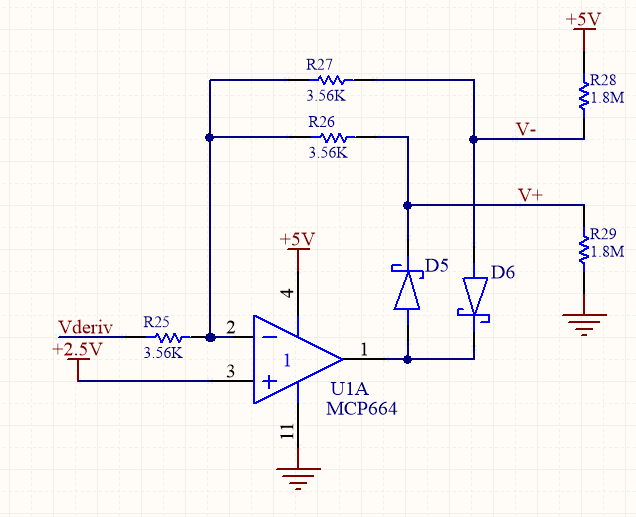
\includegraphics[scale=0.7]{Rectificador-y-restador.png}
	\caption{Rectificador y restador.}
	\label{fig:img_Rectificador_y_restador}
\end{figure}

\noindent Para poder tener finalmente la estimaci\'{o}n de la posici\'{o}n, debemos rectificar la salida del derivador alrededor de 2.5V. Esto se hace para hacer coincidir la pendiente positiva de la corriente triangular, con la pendiente negativa, y tener a la salida del estimador una se\~{n}al aproximadamente continua.

\noindent Para entender el funcionamiento de este rectificador, se comienza analizando \'{u}nicamente la etapa del primer amplificador operacional. Se parte de la suposici\'{o}n de que en un amplificador ideal, la tensi\'{o}n diferencial ($V_d$) es igual a cero. Por lo tanto, como la entrada no inversora est\'{a} fijada en 2.5V, la misma tensi\'{o}n se encuentra en la entrada inversora.

\noindent Al analizar la corriente en la resistencia $R_{25}$ (adoptando sentido positivo hacia la izquierda) en funci\'{o}n de $V_{deriv}$, resulta:

\begin{equation} \label{eq_corriente_r25}
	I_{R25}=\frac{2.5V\ -\ V_{deriv}}{R_{25}}
\end{equation}

\noindent En el caso de que $V_{deriv}$ $\mathrm{<}$ 2.5V, la corriente ser\'{a} positiva. Esta misma corriente proviene desde la salida del operacional, a trav\'{e}s del diodo D5 y por la resistencia $R_{26}$. Si se desprecia la tensi\'{o}n del diodo en directa, nos queda que la salida del operacional es igual a V+, y esta es igual a:

\begin{equation} \label{eq_V+}
	V^+=I_{R25}*R_{26}+2.5V=\frac{2.5V-V_{deriv}\ }{R25}*R_{26}+2.5V\ 
\end{equation} 

Como $R_{25}=R_{26}$

\begin{equation} \label{eq_V+_2}
	V^+\ =\ 2.5V\ -\ V_{deriv}\ +2.5V\ =\ 5V\ -\ V_{deriv}\ 
\end{equation}

An\'{a}logamente, si $V_{deriv}$ $\mathrm{>}$ 2.5V, se puede encontrar:

\begin{equation} \label{eq_V+_3}
	V^-\ =\ {5V\ -V}_{deriv}\ 
\end{equation}

Cuando D5 est\'{a} activo, $V^-=2.5\ V$ y cuando lo est\'{a} D6, $V^+\ $= 2.5 V

\subsubsection{Restador}

\noindent Se utiliza un amplificador operacional en modo diferencial como restador como se observa en la figura \ref{fig:img_Restador} y se obtiene lo siguiente.

\noindent Cuando $V_{deriv}$ $\mathrm{<}$ 2.5V:

\begin{equation} \label{eq_rest_1}
	Vestim=V^+-\ V^-\ +2.5V=\ (5V\ -\ V_{deriv})-(2.5\ V)+2.5V=5\ V\ -\ V_{deriv}\  
\end{equation}

\noindent Cuando $V_{deriv}$ $\mathrm{>}$ 2.5V: 

\begin{equation} \label{eq_rest_2}
	{Vestim=V}^+-\ V^-+2.5V=\ 2.5V\ -\ (5V-\ V_{deriv})+\ 2.5V=\ \ V_{deriv}\ 
\end{equation}

\noindent Si tomamos a $V_{deriv}$ como $V_{deriv}=\mathit{\Delta}V_{deriv}\ +\ 2,5\ V$, reemplazando en los dos casos

\noindent obtenemos que:

\begin{equation} \label{eq_rest_3}
	Vestim=\ 2,5\ V\ +\ |\mathit{\Delta}V_{deriv}|
\end{equation}

\begin{figure}[H]
	\centering
	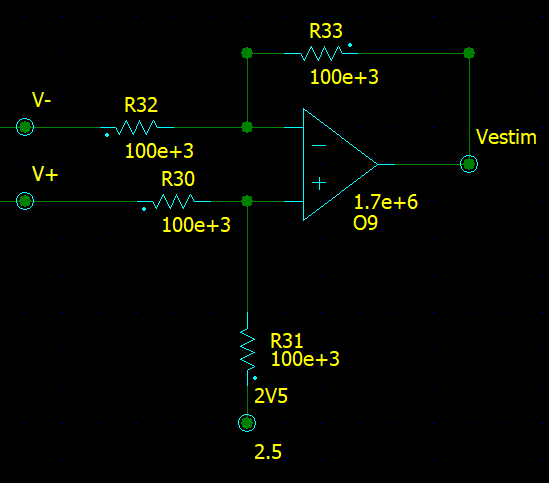
\includegraphics[scale=0.7]{Restador.png}
	\caption{Restador.}
	\label{fig:img_Restador}
\end{figure}

\subsubsection{Etapa de filtrado}

\noindent En el restador se implementa un filtrado adicional a la se\~{n}al de salida como se observa en la figura  \ref{fig:img_Esquema-circuital-del-restador-con-una-etapa-de-filtrado-en-159}. De esta \'{u}ltima etapa, considerando que $C_5=C_6=C\ $y $R_{33}=R_{31}=R$, se obtiene:

\begin{equation} \label{eq_Vestim_1}
	{Vestim}=\frac{1}{1+S*C*R}*{(V}^+-V^-\ +\ 2.5V)\ =\ \frac{1}{1+S*C*R}*(2,5\ V\ +\ |\mathit{\Delta}V_{deriv}|)
\end{equation}

\begin{equation} \label{eq_Vestim_2}
	Vestim\ =\ \frac{1}{1+S*C*R}*\ |\mathit{\Delta}V_{deriv}|\ +2.5V
\end{equation}



\noindent Puesto que la salida Vestim debe ser una continua, es importante eliminar cualquier posible ripple permitiendo solo el paso de continua. Por ello, se escogen los siguientes valores para los componentes:

\begin{enumerate}
	\item  $C=10\ nF$
	
	\item  $R=100\ Kohm$
	
	\item  $\frac{1}{2*\pi *C*R}=159.2\ Hz$
\end{enumerate}

\begin{figure}[H]
	\centering
	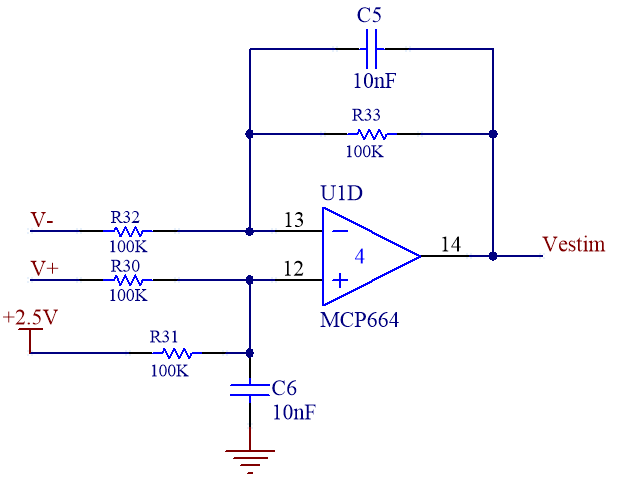
\includegraphics[scale=0.7]{Esquema-circuital-del-restador-con-una-etapa-de-filtrado-en-159.png}
	\caption{Esquema circuital del restador con una etapa de filtrado en $159.2\ Hz$.}
	\label{fig:img_Esquema-circuital-del-restador-con-una-etapa-de-filtrado-en-159}
\end{figure}

\subsection{Circuito completo}

\noindent En la figura \ref{fig:img_Circuito_estimador_de_posición_completo} se puede observar el circuito completo utilizado para la implementaci\'{o}n del rectificador, restador y filtrado.

\begin{figure}[H]
	\centering
	\includegraphics[scale=0.7]{Circuito-estimador-de-posición-completo.png}
	\caption{Circuito estimador de posición completo}
	\label{fig:img_Circuito_estimador_de_posición_completo}
\end{figure}

\subsection{Simulaci\'{o}n de estimador completo}

\noindent En la figura \ref{fig:img_Simulación_final_del_estimado} se pueden observar 3 formas de onda. La superior (verde) corresponde a la corriente del electroim\'{a}n, la del medio (amarilla) a la salida del derivador y la inferior (roja) es la salida Vestim. Utilizando cursores se midi\'{o} un ripple de 52.66mV en Vestim.

\begin{figure}[H]
	\centering
	\includegraphics[scale=0.5]{Simulación-final-del-estimador.png}
	\caption{Simulación final del estimador.}
	\label{fig:img_Simulación_final_del_estimado}
\end{figure}

\noindent En la figura \ref{tab_Resultados_de_simulación_del_estimador} se muestran valores medidos de Vestim en funci\'{o}n de la posici\'{o}n.

\begin{table}[H]
	\begin{center}
		\begin{tabular}{| c | c | c |}
			\hline
		y [mm] & L(y) [mH] & Vestim [V] \\ \hline 
		2 & 22.64 & 3.86 \\ \hline 
		3 & 18.8 & 4.13 \\ \hline 
		4 & 16.44 & 4.36 \\ \hline 
		5 & 14.9 & 4.55 \\ \hline 
		\end{tabular}
		\caption{Resultados de simulación del estimador.}
		\label{tab_Resultados_de_simulación_del_estimador}
	\end{center}
\end{table}

\subsection{Transferencia final del estimador de posici\'{o}n:}

\noindent Para la transferencia de lazo cerrado del derivador se obtiene:

\begin{equation} \label{eq_TLC_deriv_1}
	{Tlc}_{derivador}=\frac{V_{deriv}}{Vil}=\frac{-0.025*s}{1+(\frac{2*0.473}{94,5\ krad/s})*s+(\frac{s}{94,5\ krad/s})^2}
\end{equation}

\noindent De esta forma, se obtiene un sistema con un cero en el origen y dos polos complejos conjugados con una $W_n=2\pi *15000\ Hz$ y un $\xi =0.473$.

\noindent Por otro lado, al considerar el polo aportado por la etapa de restado y filtrado situado en 10 Krad/s y considerar la inversi\'{o}n de signo que genera el rectificador, se obtiene:

\begin{equation} \label{eq_TLC_deriv_2}
	\resizebox{.8\hsize}{!}
	{
	$
	{Tlc}_{estimador}=\frac{V_{estim}}{Vil}=\frac{0.025*s}{(1+\frac{s}{1\ Krad/s})*[1+(\frac{2*0.473}{94,5\ Krad/s})*s+(\frac{s}{94,5\ Krad/s})^2]}
	$
	}
\end{equation}

\noindent Para poder obtener la transferencia del diagrama en bloques: Vestim/Y:

\begin{equation} \label{eq_TLC_deriv_3}
	\resizebox{.8\hsize}{!}
	{
	$
	{Tlc'}=\frac{V_{estim}}{s*Vil}=\frac{V_{estim}}{kh*s*I_L}=\frac{0.025}{(1+\frac{s}{1\ Krad/s})*[1+(\frac{2*0.473}{94,5\ Krad/s})*s+(\frac{s}{94,5\ Krad/s})^2]}
	$
	}
\end{equation}

\noindent Como $s*I_L\equiv \frac{dI}{dt}$, se puede usar la expresi\'{o}n linealizada:

\begin{equation} \label{eq_TLC_deriv_4}
	{\left|\frac{{di}_L}{dt}\right|}_{Lineal}=\ 194690\ *\ Y[m]+676\ A/s
\end{equation}

\noindent De esta forma,  $s*I_L\equiv 194690*Y$ (sin considerar la componente de continua)

\noindent Reemplazando se obtiene:

\begin{equation} \label{eq_TLC_deriv_5}
	{Tlc'}=\frac{V_{estim}}{Y[m]}=\frac{259.6}{(1+\frac{s}{1\ Krad/s})*[1+(\frac{2*0.473}{94,5\ Krad/s})*s+(\frac{s}{94,5\ Krad/s})^2]}
\end{equation}

\noindent Considerando la etapa de filtrado de la entrada, que tiene dos polos en $2\pi *10\ KHz\ \simeq 60\ Krad/s$ se obtiene:

\begin{equation} \label{eq_TLC_deriv_6}
	\resizebox{.8\hsize}{!}
	{
		$
	{Tlc'}=\frac{V_{estim}}{Y[m]}=\frac{259.6}{(1+\frac{s}{1\ Krad/s})*{[(1+\frac{s}{60\ Krad/s})]}^2*[1+(\frac{2*0.473}{94,5\ Krad/s})*s+(\frac{s}{94,5\ Krad/s})^2]}
	$
	}
\end{equation}

\noindent Finalmente, despreciando los polos en alta frecuencia, la transferencia queda:

\begin{equation} \label{eq_TLC_deriv_7}
	{Tlc'}=\frac{V_{estim}}{Y[m]}=\frac{259.6}{(1+\frac{s}{1\ Krad/s})*{(1+\frac{s}{60\ Krad/s})}^2}
\end{equation}